\section{ラット自由行動下の軌跡のシミュレーション}
ラットが自由行動下において箱の中を探索する際の軌跡をシミュレーションする \cite{Raudies2012-gp}.これまでと異なり,現象論的に運動を生成する.場所細胞・格子細胞等自己位置と神経活動が相関する細胞のシミュレーションにおいて用いられる.
\lstinputlisting[language=julia]{./text/motor-learning/rat-trajectory/001.jl}
\lstinputlisting[language=julia]{./text/motor-learning/rat-trajectory/002.jl}
並進速度をレイリー分布,回転速度を正規分布に従うようにランダムサンプリングする.壁の接ベクトルとラットの距離を\jl{dist_wall}, 壁の法線ベクトルとラットの頭方向の角度の差を\jl{angle_wall}とする.なお,壁とはラットの自己速度ベクトルと壁全体との交点である.

\begin{itemize}
\item ラットの自己速度ベクトルと壁全体との交点を求める.
\item 交点の接ベクトルと法線ベクトルを求める.
\item 接ベクトルとの距離を\jl{dist_wall}とする.
\item 法線ベクトルと成す角を\jl{angle_wall}とする.
\end{itemize}
\lstinputlisting[language=julia]{./text/motor-learning/rat-trajectory/004.jl}
\lstinputlisting[language=julia]{./text/motor-learning/rat-trajectory/005.jl}
5分間のシミュレーションを行う.
\lstinputlisting[language=julia]{./text/motor-learning/rat-trajectory/007.jl}
黒点から始まり,赤点に終わる.
\lstinputlisting[language=julia]{./text/motor-learning/rat-trajectory/009.jl}
\begin{figure}[ht]
	\centering
	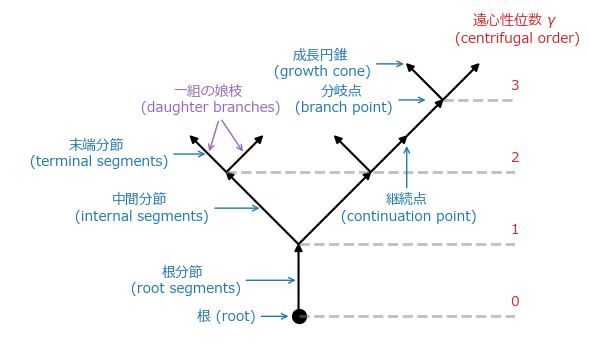
\includegraphics[scale=0.8, max width=\linewidth]{./fig/neuron-model/neurite-growth-model/cell009.png}
	\caption{cell009.png}
	\label{cell009.png}
\end{figure}
